\documentclass{beamer}
\usepackage[utf8]{inputenc}

\usetheme{Madrid}
\usecolortheme{default}
\usepackage{amsmath,amssymb,amsfonts,amsthm}
\usepackage{txfonts}
\usepackage{tkz-euclide}
\usepackage{listings}
\usepackage{adjustbox}
\usepackage{array}
\usepackage{tabularx}
\usepackage{gvv}
\usepackage{lmodern}
\usepackage{circuitikz}
\usepackage{tikz}
\usepackage{graphicx}

\setbeamertemplate{page number in head/foot}[totalframenumber]

\usepackage{tcolorbox}
\tcbuselibrary{minted,breakable,xparse,skins}



\definecolor{bg}{gray}{0.95}
\DeclareTCBListing{mintedbox}{O{}m!O{}}{%
  breakable=true,
  listing engine=minted,
  listing only,
  minted language=#2,
  minted style=default,
  minted options={%
    linenos,
    gobble=0,
    breaklines=true,
    breakafter=,,
    fontsize=\small,
    numbersep=8pt,
    #1},
  boxsep=0pt,
  left skip=0pt,
  right skip=0pt,
  left=25pt,
  right=0pt,
  top=3pt,
  bottom=3pt,
  arc=5pt,
  leftrule=0pt,
  rightrule=0pt,
  bottomrule=2pt,

  colback=bg,
  colframe=orange!70,
  enhanced,
  overlay={%
    \begin{tcbclipinterior}
    \fill[orange!20!white] (frame.south west) rectangle ([xshift=20pt]frame.north west);
    \end{tcbclipinterior}},
  #3,
}
\lstset{
    language=C,
    basicstyle=\ttfamily\small,
    keywordstyle=\color{blue},
    stringstyle=\color{orange},
    commentstyle=\color{green!60!black},
    numbers=left,
    numberstyle=\tiny\color{gray},
    breaklines=true,
    showstringspaces=false,
}
%------------------------------------------------------------
%This block of code defines the information to appear in the
%Title page
\title %optional
{4.5.14}
\date{September  2025}
%\subtitle{A short story}

\author % (optional)
{BEERAM MADHURI - EE25BTECH11012}



\begin{document}


\frame{\titlepage}
\begin{frame}{Question}
 Find the equation of the line through the point $(5, 2, -4)$ and which is parallel to the vector $3\hat{i} + 2\hat{j} - 8\hat{k}$.
\end{frame}
 
\begin{frame}{given data}
 
\begin{table}[h!]
    \centering
    \begin{tabular}{|c|c|}
\hline
\textbf{Name} & \textbf{Value} \\ \hline
$\vec{A}$ & $\myvec{2 & 1 \\0 & 3}$ \\ \hline
\end{tabular}

    \caption{4.5.14}
    \label{table 4.5.14}
\end{table}\\
   
\end{frame}

\begin{frame}{Formula}
If the direction vector of the line is $\vec{A}$ and is passing through $\vec{B}$ then, 
\begin{align*}
\text{Equation of the line is: }\vec{X} = \vec{B} +\lambda\vec{A}
 \end{align*}
 \end{frame}
\begin{frame}{solution}
    \frametitle{finding the equation of line: }
Given,
\begin{align}
\text{The line is parallel to the vector}
\begin{pmatrix}3 \\2 \\-8\end{pmatrix}
\end{align}
\begin{align}
\therefore \text{Direction vector is: } \lambda\begin{pmatrix}
3 \\
2 \\
-8
\end{pmatrix}
\end{align}

Equation of the line :-
\begin{align}
\vec{x} = \begin{pmatrix}5 \\2 \\-4\end{pmatrix} + \lambda \begin{pmatrix}3 \\2 \\-8\end{pmatrix}
\end{align}
\end{frame}
\begin{frame}
\text{Where,}
\begin{align}
\vec{x}= \begin{pmatrix}\vec{x} \\\vec{y} \\\vec{z}\end{pmatrix}
\end{align}
Hence, Equation of the line passing through $\begin{pmatrix}5 \\2 \\-4\end{pmatrix}$ and Parallel to $\begin{pmatrix}3 \\2 \\-8\end{pmatrix}$ is:\\
\begin{align*}
\vec{x} = \begin{pmatrix}5 \\2 \\-4\end{pmatrix} + \lambda \begin{pmatrix}3 \\2 \\-8\end{pmatrix}
\end{align*}
\end{frame}

\begin{frame}[fragile]
    \frametitle{Python Code}
    \begin{lstlisting}
import numpy as np
import matplotlib.pyplot as plt
from mpl_toolkits.mplot3d import Axes3D

# Point the line passes through
point = np.array([5, 2, -4])
# Direction vector
direction = np.array([3, 2, -8])

# Parameter t
t = np.linspace(-5, 5, 100)
\end{lstlisting}
\end{frame}

\begin{frame}[fragile]
\frametitle{Python Code}
\begin{lstlisting}
# Parametric equations of the line
x = point[0] + direction[0] * t
y = point[1] + direction[1] * t
z = point[2] + direction[2] * t

# Create the figure
fig = plt.figure(figsize=(8, 6))
ax = fig.add_subplot(111, projection='3d')
# Plot the line
ax.plot(x, y, z, color='blue', label='Line through (5,2,-4) parallel to (3,2,-8)')
    \end{lstlisting}
\end{frame}

\begin{frame}[fragile]
    \frametitle{Python Code}
    \begin{lstlisting}
# Highlight the given point
ax.scatter(point[0], point[1], point[2], color='red', s=50, label='Point (5,2,-4)')

# Axis labels and title
ax.set_xlabel('X')
ax.set_ylabel('Y')
ax.set_zlabel('Z')
ax.set_title('3D Line Plot')
ax.legend()

plt.show()
    \end{lstlisting}
\end{frame}



\begin{frame}[fragile]
\frametitle{C Code}
\begin{lstlisting}
#include <stdio.h>

int main() {
    // Point through which the line passes
    double x0 = 5, y0 = 2, z0 = -4;
    // Direction vector
    double a = 3, b = 2, c = -8;

    printf("The vector equation of the line is:\n");
    printf("r = (%.1f, %.1f, %.1f) + t(%.1f, %.1f, %.1f)\n", x0, y0, z0, a, b, c);
\end{lstlisting}
\end{frame}

\begin{frame}[fragile]
\frametitle{C Code}
\begin{lstlisting}
    printf("\nParametric form:\n");
    printf("x = %.1f + %.1f t\n", x0, a);
    printf("y = %.1f + %.1f t\n", y0, b);
    printf("z = %.1f + %.1f t\n", z0, c);

    return 0;
}
\end{lstlisting}
\end{frame}

\begin{frame}[fragile]
\frametitle{Python and C Code}
\begin{lstlisting}
import subprocess
import os

# Determine the executable name based on the operating system
executable_name = 'line_program'
if os.name == 'nt':  # 'nt' is the name for Windows
    executable_name += '.exe'
# Prepend './' to specify the current directory
executable_path = os.path.join('.', executable_name)
\end{lstlisting}
\end{frame}

\begin{frame}[fragile]
\frametitle{Python and C Code}
\begin{lstlisting}
    # Run the C program as a subprocess
    # capture_output=True saves its output
    # text=True decodes the output as text
    # check=True raises an error if the C program fails
    result = subprocess.run(
        [executable_path],
        capture_output=True,
        text=True,
        check=True
    )
    # Print the output that was captured from the C program
    print(result.stdout)
\end{lstlisting}
\end{frame}
\begin{frame}
\begin{figure}
    \centering
    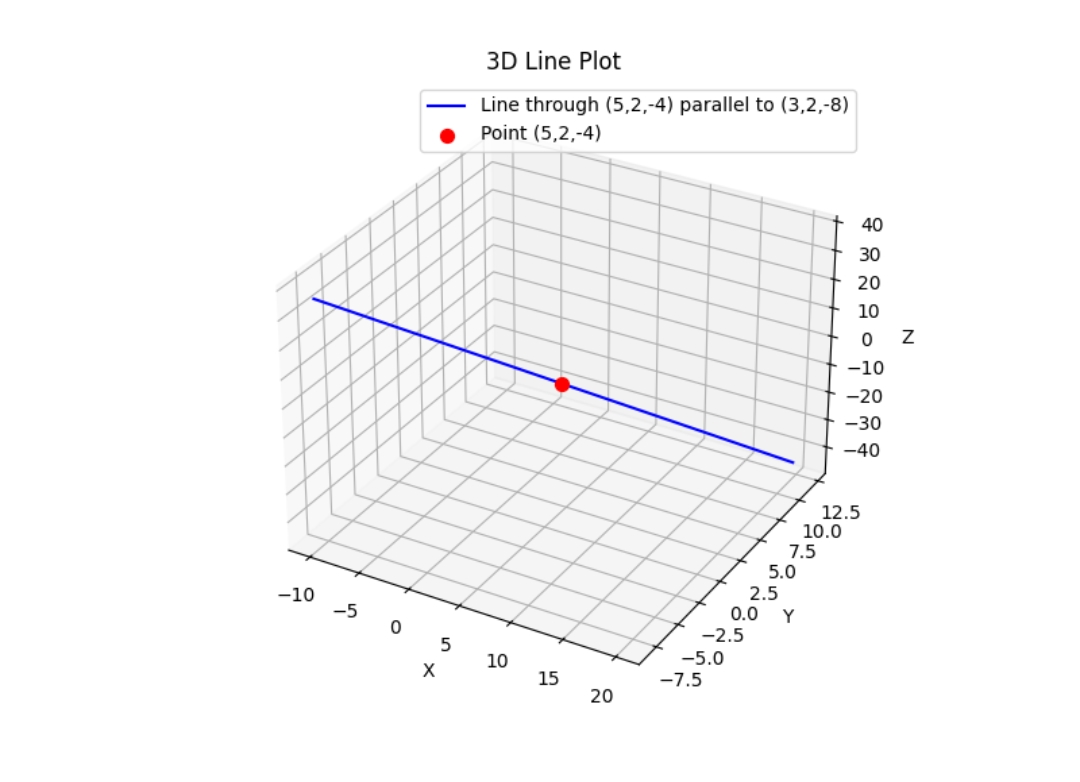
\includegraphics[width=0.75\columnwidth]{line.jpg}
    \caption{Plot}
    \label{fig:Line}
\end{figure}
\end{frame}

\end{document}